\begin{frame}
\frametitle{Megoldás}

\begin{center}
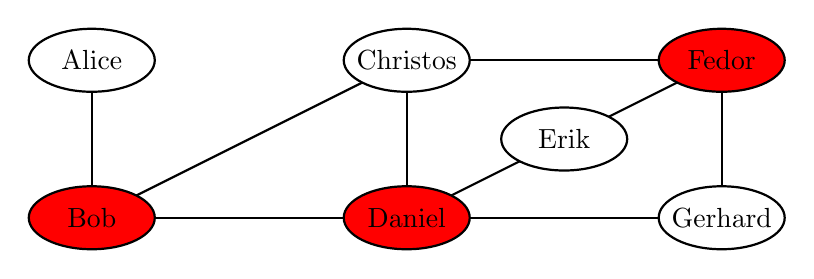
\begin{tikzpicture}[scale=2]
\coordinate (A) at (1,2);
\coordinate (B) at (1,1);
\coordinate (C) at (3,2);
\coordinate (D) at (3,1);
\coordinate (E) at (4,1.5);
\coordinate (F) at (5,2);
\coordinate (G) at (5,1);

\draw[thick] (B) -- (D);
\draw[thick] (D) -- (G);
\draw[thick] (C) -- (F);

\draw[thick] (B) -- (A);
\draw[thick] (D) -- (C);
\draw[thick] (G) -- (F);

\draw[thick] (B) -- (C);
\draw[thick] (D) -- (E);
\draw[thick] (E) -- (F);

\draw[thick, fill=white] (A) ellipse (0.4 and 0.2) node {Alice};
\draw[thick, fill=red  ] (B) ellipse (0.4 and 0.2) node {Bob};
\draw[thick, fill=white] (C) ellipse (0.4 and 0.2) node {Christos};
\draw[thick, fill=red  ] (D) ellipse (0.4 and 0.2) node {Daniel};
\draw[thick, fill=white] (E) ellipse (0.4 and 0.2) node {Erik};
\draw[thick, fill=red  ] (F) ellipse (0.4 and 0.2) node {Fedor};
\draw[thick, fill=white] (G) ellipse (0.4 and 0.2) node {Gerhard};
\end{tikzpicture}
\end{center}

\begin{footnotesize}
\begin{itemize}
\item Csúcsok = vendégek, élek = verekedni fognak.
\item Kitilható vendégek száma: k=3.
\end{itemize}
Kérdések:
\begin{itemize}
\item Kit tiltsunk ki, hogy ne legyen verekedés? \\
\textcolor{red}{Bob-ot, Daniel-t és Fedor-t.}
\item Melyik Algoritmuselméletből tanult feladat ez? \\
\textcolor{red}{k elemű lefogó csúcshalmaz: $\forall$ él legalább egyik végpontja benne van.}
\end{itemize}
\end{footnotesize}
\end{frame}

